\documentclass{article}

%Added this for math
\usepackage{amsmath}
\usepackage{amssymb}
\usepackage{graphicx}
\usepackage{graphics}
\usepackage{multirow}
\usepackage{multicol}
\usepackage{epsfig}
\usepackage[table,xcdraw,svgnames,dvipsnames]{xcolor}
\usepackage{Revised_version/tikz-related}
\usepackage{float}
\newcommand{\abs}[1]{\left\lvert #1 \right\rvert} %this makes it easier to use absolute bars (now /abs{})
% ---------------------------------

	\def\papertitle{Generating Synthetic Vehicle Data Using Decentralized Generative Adversarial Networks (T-IV-23-05-0965)}
	\def\authors{B.~Shaker, G.~P.~Rosati~Papini, M.~Saveriano, and K.-Y.~Liang}
	
	\def\Editor{Dear Professor Fei-Yue Wang\\}
	
	\def\Letter{Enclosed please find the replies to the Editor's and Reviewers' comments with a detailed statement of changes made in order to address those comments. We also attached a PDF file that highlights the changes in the revised version of the paper with respect to the previous version, where the blue colour marks the revised text.
	\\ \\
	Best regards,\\
	\\
	G. P. Rosati Papini
}


\providecommand{\lettertitle}{Author Response to Reviews of}
\providecommand{\papertitle}{Title}
\providecommand{\authors}{Authors}
\providecommand{\journal}{Journal}
\providecommand{\doi}{--}
\providecommand{\Editor}{Name}
\providecommand{\Letter}{Body}

\usepackage[includeheadfoot,top=10mm, bottom=10mm, footskip=2.5cm]{geometry}


% Typography
\usepackage[T1]{fontenc}
\usepackage{times}
%\usepackage{mathptmx} % math also in times font
\usepackage{amssymb,amsmath}
\usepackage{microtype}
\usepackage[utf8]{inputenc}
\usepackage{bm,times} % assumes new font selection scheme installed

% Misc
\usepackage{graphicx}
\usepackage[hidelinks]{hyperref} %textopdfstring from pandoc
\usepackage{soul} % Highlight using \hl{}

\usepackage{caption}
\usepackage{subcaption}
\usepackage{graphics} % for pdf, bitmapped graphics files
\usepackage{epsfig} % for postscript graphics files
\graphicspath{{../figs/}}
\usepackage{epstopdf}
\usepackage{stfloats}

% Table

\usepackage{adjustbox} % center large tables across textwidth by surrounding tabular with \begin{adjustbox}{center}
\renewcommand{\arraystretch}{1.5} % enlarge spacing between rows
\usepackage{caption} 
\captionsetup[table]{skip=10pt} % enlarge spacing between caption and table
\usepackage{multirow}
\usepackage{booktabs}
% Section styles

\usepackage{titlesec}
\titleformat{\section}{\normalfont\Large}{\makebox[0pt][r]{\bf \thesection.\hspace{4mm}}}{0em}{\bfseries}
\titleformat{\subsection}{\normalfont}{\makebox[0pt][r]{\bf \thesubsection.\hspace{4mm}}}{0em}{\bfseries}
\titlespacing{\subsection}{0em}{1em}{-0.3em} % left before after

% Paragraph styles

\setlength{\parskip}{0.6\baselineskip}%
\setlength{\parindent}{0pt}%


% Quotation styles
\usepackage{framed}
\let\oldquote=\quote
\let\endoldquote=\endquote
\renewenvironment{quote}{\begin{fquote}\itshape\advance\leftmargini -2.4em\begin{oldquote}}{\end{oldquote}\end{fquote}}

%\usepackage{xcolor}
%\newenvironment{fquote}
%  {\def\FrameCommand{
%	\fboxsep=0.6em % box to text padding
%	\fcolorbox{blue}{white}}%
%	% the "2" can be changed to make the box smaller
%    \MakeFramed {\advance\hsize-2\width \FrameRestore}
%    \begin{minipage}{\linewidth}
%  }
%  {\end{minipage}\endMakeFramed}

\usepackage{xcolor}
\newenvironment{fquote}
{\def\FrameCommand{
		\fboxsep=0.6em % box to text padding
		\fcolorbox{blue}{white}}%
	% the "2" can be changed to make the box smaller
	\MakeFramed {\advance\hsize-3\width \FrameRestore}
	}
	{\endMakeFramed}

% Table styles

\let\oldtabular=\tabular
\let\endoldtabular=\endtabular
\renewenvironment{tabular}[1]{\begin{adjustbox}{center}\begin{oldtabular}{#1}}{\end{oldtabular}\end{adjustbox}}


% Shortcuts

%% Let textbf be both, bold and italic
%\DeclareTextFontCommand{\textbf}{\bfseries\em}

%% Add RC and AR to the left of a paragraph
%\def\RC{\makebox[0pt][r]{\bf RC:\hspace{4mm}}}
%\def\AR{\makebox[0pt][r]{AR:\hspace{4mm}}}

%% Define that \RC and \AR should start and format the whole paragraph 

\newcounter{RCcounter}
\setcounter{RCcounter}{0}
\newcounter{Rcounter}
\setcounter{Rcounter}{0}

\usepackage{suffix}
\long\def\RC#1\par{\makebox[0pt][r]{\bf RC\arabic{Rcounter}\arabic{RCcounter}:\hspace{4mm}}\textbf{{#1}}\par} %\RC
\WithSuffix\long\def\RC*#1\par{\textbf{{#1}}\par} %\RC*
\long\def\AR#1\par{\makebox[0pt][r]{AR\arabic{Rcounter}\arabic{RCcounter}:\hspace{10pt}}{\textcolor{blue}{#1}}\stepcounter{RCcounter}\par} %\AR
\WithSuffix\long\def\AR*#1\par{{#1}\par} %\AR*


\def\headall{
\setcounter{RCcounter}{1}
{\Large\bf \lettertitle}\\[1em]
{\Large \papertitle}\\[1em]
{\authors}\\
%{\it \journal, }\texttt{doi:\doi}\\
\hrule
% Legend
\hfill {\bfseries RC:} \textbf{{Reviewer Comment}},\(\quad\) AR: \textcolor{blue}{Author Response}, \(\quad\textcolor{blue}{\square}\) \emph{\textcolor{blue}{Manuscript text}}
\stepcounter{Rcounter}}


%%%
%DIF PREAMBLE EXTENSION ADDED BY LATEXDIFF
%DIF UNDERLINE PREAMBLE %DIF PREAMBLE
\RequirePackage[normalem]{ulem} %DIF PREAMBLE
\RequirePackage{color}\definecolor{RED}{rgb}{1,0,0}\definecolor{BLUE}{rgb}{0,0,1} %DIF PREAMBLE
\providecommand{\DIFadd}[1]{{\protect\color{blue}\uwave{#1}}} %DIF PREAMBLE
\providecommand{\DIFdel}[1]{{\protect\color{red}\sout{#1}}}                      %DIF PREAMBLE
%DIF SAFE PREAMBLE %DIF PREAMBLE
\providecommand{\DIFaddbegin}{} %DIF PREAMBLE
\providecommand{\DIFaddend}{} %DIF PREAMBLE
\providecommand{\DIFdelbegin}{} %DIF PREAMBLE
\providecommand{\DIFdelend}{} %DIF PREAMBLE
%DIF FLOATSAFE PREAMBLE %DIF PREAMBLE
\providecommand{\DIFaddFL}[1]{\DIFadd{#1}} %DIF PREAMBLE
\providecommand{\DIFdelFL}[1]{\DIFdel{#1}} %DIF PREAMBLE
\providecommand{\DIFaddbeginFL}{} %DIF PREAMBLE
\providecommand{\DIFaddendFL}{} %DIF PREAMBLE
\providecommand{\DIFdelbeginFL}{} %DIF PREAMBLE
\providecommand{\DIFdelendFL}{} %DIF PREAMBLE
%DIF END PREAMBLE EXTENSION ADDED BY LATEXDIFF

% Highlight
\newcommand{\highlight}[2][yellow]{\mathchoice%
	{\colorbox{#1}{$\displaystyle#2$}}%
	{\colorbox{#1}{$\textstyle#2$}}%
	{\colorbox{#1}{$\scriptstyle#2$}}%
	{\colorbox{#1}{$\scriptscriptstyle#2$}}}%

 \usepackage{pdfpages}
 
\newcommand{\sqboxEmpty}[1]{%
	\colorbox{#1}{\Square}%
}%


\begin{document}
{\Large\bf \Editor}\\[1em]
{\large\Letter}\\[1em]
\newpage
% Make title
\headall


\section{Editor}

\RC I believe the topic of your paper is interesting and beneficial to TIV, therefore I would like to invite you to revise thoroughly according to our review reports, and resubmit your revision as a New paper. If you do so, please let me know before your submission and provide me with a detailed report on your revision, I will let you know my opinion.

\AR We thank the Editor for appreciating our work and for guiding the revision. In the revised version, we have addressed all the comments from the reviewers. Please find the detailed answers below.

%\RC comment

%\AR Please refer to the individual reviewer replies for details.


\newpage
% Make title
\headall

\section{Reviewer \#1}

\RC The writing quality of this paper is poor, there are many writing mistakes that can be seen throughout the paper. For instance, P2, L47, LSTM, The author should provide the full name when an abbreviation is first used.

\AR We thank the reviewer for the careful reading of the manuscript. To comply with the request, we have clarified all abbreviations in the text when they are used for the first time.
We have also subjected the manuscript to careful proofreading using Grammarly software. 

%TODO: 
%\begin{itemize}
%    \item Include all and every abbreviation into the glossary even if it is very obvious.
%    \item Use grammarly (or similar) on all paragraphs after finishing the editing. 
%\end{itemize}

\begin{quote}
    We careful proofreading all the document.
\end{quote}

\RC The authors need to emphasise their contributions/novelties in introduction. In the current version, the authors provide too much unnecessary details or background information. Authors should give detailed references and lines of research development A well-written introduction should provide a clear and concise summary of the main points and contributions of the paper.

\AR We thank the reviewer for the suggestion, which we find useful and necessary. We have done our best to remove all unnecessary details from the manuscript and tried to make our contribution more obvious, which in particular focuses on the following points, which we will also mention here in the answer for completeness:
    \begin{enumerate}
        \item Our model can effectively learn from multiple non-IID time-series and converge to a solution that fools all discriminators. Experimental results show that our approach outperforms existing centralized methods, such as TimeGAN, for non-IID time-series in terms of the quality of the generated synthetic data.
        \item We present a novel discriminator architecture, based on CNNs, that facilitates the generation of sequences with variable lengths. To accommodate sequences of diverse lengths, we incorporate an adaptive pooling layer within the discriminator. This enhancement augments the generator's capability to accurately reproduce sequences of varying lengths.
        \item We propose a novel normalization technique to further enhance the training process. More in details, the server determines the global minimum and maximum values for each feature, considering the lowest minimum and the highest maximum values received from all the workers. These global boundaries are then sent back to all workers for normalization of their local data. We experimentally show that this approach outperforms the normalization based on the known range of the specific sensors involved.
        \end{enumerate}

%\begin{itemize}
%    \item Rewrite the intro to really emphasize our contributions, which are as follows:
%    \begin{enumerate}
%        \item Our model can effectively learn from multiple non-IID time- series and converge to a solution that fools all discriminators. Experimental results show that our approach outperforms existing centralized methods, such as TimeGAN, for non- IID time-series in terms of the quality of the generated synthetic data  
%        \item We present a novel discriminator architecture, based on CNNs, that facilitates the generation of sequences with variable lengths. To accommodate sequences of diverse lengths, we incorporate an adaptive pooling layer within the discriminator. This enhancement augments the generator's capability to accurately reproduce sequences of varying lengths.
%        \item We propose a novel normalization technique to further enhance the training process. More in details, the server determines the global minimum and maximum values for each feature, considering the lowest minimum and the highest maximum values received from all the workers. These global boundaries are then sent back to all workers for normalization of their local data. We experimentally show that this approach outperforms the normalization based on the known range of the specific sensors involved.
%        \end{enumerate}
%    \item Complaining about unnecessary details might be due to including previous works into introduction. Suggest re-separating it into its own section.
%\end{itemize}

\begin{quote}
	We have changed the introduction by making our contribution immediately clear. We added the Figure~6 the show one of our contribution.
\end{quote}

\RC The authors are suggested to carefully rephrase the format of each cited reference in the manuscript to ensure a better writing quality. The author needs to unify all writing formats.

\AR We thank the reviewer for the suggestion. We have reviewed and rechecked all citations.
%\begin{itemize}
%    \item I think the complaint is for how we put the reference in the text and not the actual formatting of the references? unclear
%\end{itemize}

\begin{quote}
	We have fixed all wrong citations and aligned the formats.
\end{quote}

\RC The images in the font size is too small. Fig. 1. makes it difficult for the reader to understand.

\AR Thanks for the advice, we improved the legibility of the figure~1 by enlarging the character and improving the appearance.
%\begin{itemize}
%    \item Redone Fig.1 specifically. made it page width, increased fontsize, changed color-coding, added more info in the caption.
%    \item Should we do the same for the rest of the figures?
%\end{itemize}

\begin{quote}
    Redone Fig.1 specifically. made it page width, increased fontsize, changed color-coding, added more info in the caption.
\end{quote}

\RC The authors claim that the generated features maintained the same correlations exhibited in the real data. They should prove this idea with more experiments and metrics. For instance, metric: FID, KID, IS, etc.

\AR We appreciate the reviewer's comment. FID, KID, and IS are generally used for evaluating the quality and diversity of images produced by GANs. They rely on using a pretrained model, like Inception v3, which was trained on images, to extract features from the generated and real data. Therefore, these metrics aren't directly applicable to time series data. In our manuscript, we presented an auto-regression model and have instead used R-squared (R2), Mean Absolute Error (MAE), and Root Mean Squared Error (RMSE) as part of our evaluation methodology to compare our generated time-series data with the real data. However, we have performed earlier tests with the GAN model on images before adapting it to time-series data, which were omitted from the manuscript as we wanted it to be very specific to vehicle sensor data.
\\
We trained nine different decentralized training strategies, which were as follows: 
\setlength{\columnsep}{-3cm}
\begin{multicols}{2}[\small]
\begin{enumerate}
    \item Most Forgiving
    \item Least Forgiving
    \item Most Forgiving - Override
    \item Least Forgiving - Override
    \item Weighted Average - Most Forgiving
    \item Weighted Average - Least Forgiving
    \item Weighted Average - Most Forgiving [different Learning Rates]
    \item Weighted Average - Most Forgiving [3:1 D to G training]
    \item Weighted Average - Least Forgiving [3:1 D to G training]
    \item[]
\end{enumerate}
\end{multicols}
\\
To decide on the best decentralized training strategy, all the trained generator models were saved at epoch number 200. Each generator's output was tested by calculating the FID score for 10 epochs. To level out the playing field across all generators, a random noise is produced and used by each generator to create fake images during each epoch. Furthermore, the same random set of real images are also used to calculate the FID score using the Inception network.
\\
The results depicted in Figure -- demonstrate that, among tested generators, generator number two (the least forgiving) performed the best. Both qualitative and quantitative evaluation metrics indicated that the least forgiving discriminator outperformed the other proposed strategies.

\def\genbarscaley{0.5}
\def\genbarscalex{0.8}
\begin{figure}[H]
    \centering
\begin{tikzpicture}[line width = 1pt,line cap=round, line join=round,anchor=center]  
    
\begin{axis}[
    ybar, 
    bar width=20pt,
    ylabel={FID Score},
    xlabel={Generator Number},
    xtick=data,
    ymin = 20,
    % ymax= 235,
    axis x line*=bottom,
    axis y line=left,
    axis line style={-,line width = 1pt},
    width=\genbarscalex\textwidth,
    height=\genbarscaley\textwidth,
    error bars/y dir=both,
    error bars/y explicit,
    error bars/error bar style={
      line width = 1 pt,
      color=black
    },
    nodes near coords,
    every node near coord/.style={
        font=\bfseries,
        color=white,
        anchor=east,
        rotate=90,
        },
    ]
\addplot [fill=myblue ,line width = 1pt] table [
    col sep=comma,
    header=true,
    x=gen, 
    y=mean, 
    y error=sd,
    ] {Reply_to_comments/gen_mean_sd.csv};
    
\end{axis}    
\end{tikzpicture}
    \caption{FID mean score results for the nine generators}
    \label{fig:gen-bargraph}
\end{figure}

\begin{quote}
We have better justified the use of an auto-regressive model to evaluate performance through the R2, MAE and RMSE indices by rewriting the introduction of the paragraph \textbf{IV.C Evaluation matrics}.
\end{quote}

\RC In the experiment, the author should give more details including but not limited to: dataset, training strategy, training tricks, etc. The experimental setup of datasets is not clear.

\AR We thank the reviewer for verifying the absence of some important information and we now provide all necessary information.
In particular, we employ the Adam optimizer with a learning rate of 2e-4, and parameters $\beta1$ = 0.5, $\beta2$ = 0.999 for both generator and discriminator.
We found that \gls*{mse} loss outperformed \gls*{bce}, especially in a decentralized setting. The noise dimension for the generator was set to 128 and the batch size used was 4. 
Our testing showed that in our decentralized training setup, overriding the models with the winning discriminator led to a degradation in performance. Therefore, the chosen worker does not override the other workers.

%\begin{itemize}
%    \item These info are all within the original thesis report. We need to revisit adding those back and expanding on what we have in the publication. The question now is, how many pages will this add? what is our new page count target?
%\end{itemize}

\begin{quote}
We have added the above information by rewriting paragraph \textbf{IV.C Decentralised Training Sequence}
\end{quote}

\RC In section IV, more ablation studies should be added to analyze the design of the Generative Adversarial networks and Federated Learning, such as the effects of different kinds of loss and training strategies?

\AR To realise a work with these characteristics, an ablation studies is a must. For this reason, we conducted a series of preliminary ablation studies specifically for image-based GANs before adapting it to time-series data. In particular we studied:
\begin{itemize}
    \item The effects of different loss functions, particularly MSE and BCE. In a centralized setup, there were no major difference between the performance of BCE and MSE loss, however, MSE performed significantly better than BCE. 
    \item The impact of batch size on the performance of the image-based GANs. The network was able to learn much faster using a smaller batch size of 16 compared to 64. Both the image output and the FID score confirm that the output improved with a smaller size batch given a larger number of workers and limited local data.
    \item The effect of the learning rate on the weighted average of the most and least forgiving strategies. We experimented with different learning rates for the discriminator and generator, specifically increasing the discriminator learning rate to 0.002. Additionally, we adjusted the discriminator-generator training ratio to 3:1. Despite these modifications, the changes resulted in image output degradation.
\end{itemize}
Obviously, these tests carried out on image-based GANs have been omitted for reasons of space in the final discussion, limiting ourselves to presenting the final studies carried out directly on time-series more in detail as more interesting and specific in our work.
In particular we report:
\begin{itemize}
    \item The effect of the dynamic window reported in Table~II.
    \item The effect of worker normalization, Table~III.
    \item The effect of Federated Learning strategy, Table~IV.
\end{itemize}

%\begin{itemize}
%\item We conducted a series of ablation studies specifically for image-based GANs before adapting it to time-series data. These studies were not applied to time-series GANs as it was already proved by the image-based GANs studies.
%\item We analyzed the effects of different loss functions, particularly MSE and BCE. In a centralized setup, there were no major difference between the performance of BCE and MSE loss, however, MSE performed significantly better than BCE. 
%\item We also examined the impact of batch size on the performance of the GANs. The network was able to learn much faster using a smaller batch size of 16 compared to 64. Both the image output and the FID score confirm that the output improved with a smaller size batch given a larger number of workers and limited local data.
%\item Furthermore, we studied the effect of the learning rate on the weighted average of the most and least forgiving strategies. We experimented with different learning rates for the discriminator and generator, specifically increasing the discriminator learning rate to 0.002. Additionally, we adjusted the discriminator-generator training ratio to 3:1. Despite these modifications, the changes resulted in image output degradation.
%\end{itemize}
%
% TODO: 
% \begin{itemize}
%     \item Same as previous point. The original report, specifically in the image-based, had a section about (MSE vs BCE), (effect of batch size), (learning rate effect on weighted average most/least forgiving).
%     \item Which ones to include? this is a lot of information. Suggest MSE vs BCE and batch size?
%     \item add more details in the response, then add a small info in the report
% \end{itemize}

\begin{quote}
    We have added concisely information on the chosen strategy and motivation in the section \textbf{IV.C Decentralised Training Sequence}
\end{quote}


\newpage
\headall

\section{Reviewer \#2}

\RC The novelty of this paper is limited. Both the network architecture and the deployment of the federated learning approach are commonly used in related works. The contribution of the paper should be strengthened and highlighted.

\AR  We thank the reviewer for the warning, which we find useful and necessary. We have done our best to make our contribution more obvious, modify the introduction. We report the contribution here in the answer for completeness:
    \begin{enumerate}
        \item Our model can effectively learn from multiple non-IID time-series and converge to a solution that fools all discriminators. Experimental results show that our approach outperforms existing centralized methods, such as TimeGAN, for non-IID time-series in terms of the quality of the generated synthetic data.
        \item We present a novel discriminator architecture, based on CNNs, that facilitates the generation of sequences with variable lengths. To accommodate sequences of diverse lengths, we incorporate an adaptive pooling layer within the discriminator. This enhancement augments the generator's capability to accurately reproduce sequences of varying lengths.
        \item We propose a novel normalization technique to further enhance the training process. More in details, the server determines the global minimum and maximum values for each feature, considering the lowest minimum and the highest maximum values received from all the workers. These global boundaries are then sent back to all workers for normalization of their local data. We experimentally show that this approach outperforms the normalization based on the known range of the specific sensors involved.
        \end{enumerate}

%\begin{itemize}
%    \item Don't know how to address the concern about limited novelty. Would re-writing the introduction be sufficient?
%\end{itemize}

\begin{quote}
    We have changed the introduction by making our contribution immediately clear. We added the Figure~6 the show one of our contribution.
\end{quote}

\clearpage
\RC Comparison with related FL-based GANs is lacking, which makes it hard to assess the superiority of the proposed method.

\AR We understand the reviewer's concern. As we were previously aware, there are no works with comparable characteristics. In order to overcome this weakness, as suggested by the reviewer, we have decided to compare ourselves with the work presenting TimeGANs even though this is not implemented in a decentralised manner. We report the table here for completeness of the results.
\\\\\\
\begin{tabular}{l|ccc|ccc}
\hline
Approaches &
  \multicolumn{3}{c}{\sc{TRTS}} &
  \multicolumn{3}{c}{\sc{TSTR}} \\
  \hline
 &
  \sc{R2} &
  \sc{MAE} &
  \sc{RMSE} &
  \sc{R2} & 
  \sc{MAE} &
  \sc{RMSE} \\ 
  \hline
Our approach (dynamic window)     & 0.550 & 0.070 & 0.171 & 0.621 & 0.051 & 0.162\\ 
\hline
TimeGAN     & 0.471	& 0.073	& 0.187	& 0.604	& 0.057	& 0.162\\ 
\hline
\end{tabular}%
\\\\\\
We conducted PCA analysis, which were omitted from the report due to space constraints, and the fact that results from TimeGAN is not quite relevant to the main body of the report. Here is a comparison of the PCA of our best performer, the least forgiving Decentralized model, vs. the centralized TimeGAN showing that our model were more successful in capturing the data distribution, while TimeGAN showed distributions that were not present in the real data:
\def\batchscale{0.5}
\def\batchyscale{0.3}
\def\batchcol{myblue}
\def\batchtcol{orange}
\def\markersize{0.6}

\begin{figure} [htp]
    \centering
    \subfloat[Least Forgiving]{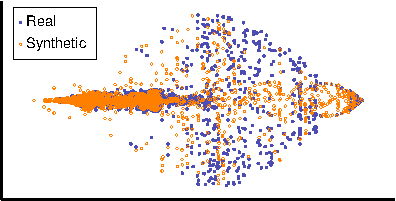
\includegraphics[scale=1]{Revised_version/Images/pca-lf.pdf}} \hspace{0.9 cm}
\subfloat[TimeGAN]{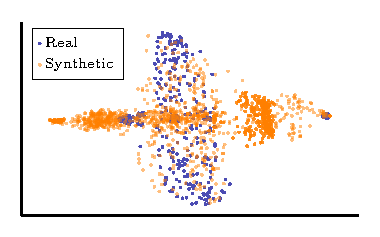
\includegraphics[scale=1]{Revised_version/Images/pca-timegan.pdf}} 
    \caption{PCA output of Decentralized least forgiving vs. centralized TimeGAN}
    \label{fig:timegan-pca}
\end{figure}

%TODO: 
%\begin{itemize}
%    \item Unsure how to tackle this concern. Currently, there are no time-series based Decentralized GANs on the market to compare it to. This was an image-based that was adapted based on an earlier decision taken at the beginning of the thesis.
%    \item We included the most similar in the results, which was TimeGAN, but its not decentralized.
%\end{itemize}

\begin{quote}
    We added a line on the Table~II related to the TimeGAN and we comment in the text Section \textbf{V.A Centralized GAN Results}.
\end{quote}

\RC A brief survey of related works on federated learning and GANs should be added. Besides, the usage of FL-based GANs in intelligent vehicles should be also be introduced and summarized.

\AR Thanks for the note. We have improved the quality of the related works, in particular by adding a specific section where some related works are presented.
In particular we present some different approaches as F2U, F2A, FeGANs, EFFGAN for the FL; and the TimeGAN for the time-series.
In terms of FL-based GANs in intelligent vehicles, we cannot find something that directly translates to our application. The intersection of Federated Learning, GANs, and intelligent vehicles is highly specific.

%\begin{itemize}
%    \item We included F2U, F2A, FeGANs, EFFGAN. I guess we need to include more? I can add FeTGAN, which is based on TimeGAN.
%    \item In terms of FL-based GANs in intelligent vehicles. I cannot find something that directly translates to our application. The intersection of Federated Learning, GANs, and intelligent vehicles is highly specific. The most closest thing i found was this, but its image based and not decentralized: \href{https://openaccess.thecvf.com/content/WACV2021W/AVV/papers/Xu_Reliability_of_GAN_Generated_Data_to_Train_and_Validate_Perception_WACVW_2021_paper.pdf}{\textbf{[LINK]}}
%\end{itemize}

\begin{quote}
	We added the Section \textbf{II Related Works}
\end{quote}



\end{document}